Given : $\triangle{ABC}$
, $\vec{D}$,$\vec{E}$ and $\vec{F}$ are the midpoints of AB,BC and CA respectively

\begin{figure}[!ht]
\centering
\resizebox{\columnwidth}{!}{%
%
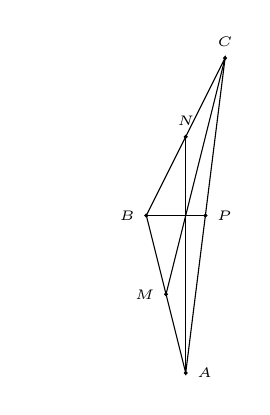
\begin{tikzpicture}
%[scale=0.5,>=stealth,point/.style={draw,circle,fill = green,inner sep=0.1pt},]
[scale=0.5,>=stealth, point/.style={draw,circle,fill = black,inner sep=0.1pt}]


%%
%%%Triangle sides
\def\a{4.12}
\def\b{4.47}
%\def\c{sqrt(\a^2+\c^2)}
\def\c{8.06}
%%
%%
%%
%%%Labeling points
%\node (A) at (0,\b)[point,label=above right:$A$] {};
%\node (B) at (\a, 0)[point,label=below left:$B$] {};
%\node (C) at (0, 0)[point,label=below right:$C$] {};
%\node (M) at (\a*0.5,\b*0.5)[point,label=above:$M$] {};
%\node (D) at (\a,\b)[point,label=above right:$D$] {};
%%
%%
%%%Drawing triangle ABC
%\draw (A) -- node[below] {$\textrm{}$} (B) -- node[left] {$\textrm{a}$} (C) -- node[above,xshift=5mm] {$\textrm{b}$} (A);
%%
%%%Joining CD
%\draw (C)--(D);
%%%Joining BD
%\draw (B)--(D);
%%
%%%Drawing and marking angles
%%\tkzMarkAngle[fill=orange!40,size=0.5cm,mark=](A,M,C)
%%\tkzMarkAngle[fill=orange!40,size=0.5cm,mark=](B,M,D)
%%\tkzMarkAngle[fill=green!40,size=0.5cm,mark=](A,B,C)
%%\tkzMarkRightAngle[fill=blue!20,size=.2](A,C,B)
%%\tkzMarkRightAngle[fill=blue!20,size=.2](D,B,C)
%%\tkzLabelAngle[pos=0.65](A,M,C){$\theta$}
%%\tkzLabelAngle[pos=0.65](B,M,D){$\theta$}
%%\tkzLabelAngle[pos=0.65](A,B,C){$\alpha$}
%%


% the coordinates of the vertices
\coordinate (A) at (4,-6);
\coordinate (B) at (3,-2);
\coordinate (C) at (5,2);


\coordinate (M) at (3.5,-4);
\coordinate (N) at (4,0);
\coordinate (P) at (4.5,-2);

% the axis
\draw[thin,scale=0,-] (-1,0) -- (5.5,0);
\draw[thin,scale=0,-] (0,-2.5) -- (0,2.5);

% the edges of the triangle
\draw (A) -- (B) -- (C) -- cycle;
\draw[-] (B) -- (P) ;
\draw[-] (A) -- (N) ;
\draw[-] (C) -- (M) ;

% labelling the vertices
%\node (A) at (4,-6)[point,label=above right:$A$] {};
\node[point,label={right:\tiny $A$}] at (A) {};
\node[point,label={left:\tiny $B$}] at (B) {};
\node[point,label={above:\tiny $C$}] at (C) {};
\node (M) at (3.5,-4)[point,label=left:\tiny $M$]{};
\node (N) at (4,0)[point,label=above:\tiny $N$] {};
\node (P) at (4.5,-2)[point,label=right:\tiny $P$] {};

% the arcs for the angles
%\begin{scope}[black]
%\draw[->]
%  (1,0) +(0:0.5cm) arc [radius=1cm,start angle=0,end angle=41] node[midway,right] {$\alpha$};
%\draw[->]
%  (0.5,0) +(0:0.25cm) arc [radius=0.75cm,start angle=0,end angle=122] node[midway,above] {$\beta$};
%\end{scope}
%
\end{tikzpicture}
%



%\begin{tikzpicture}[scale=.5]
%  \tkzDefPoint(4,-6){A} \tkzDefPoint(3,-2){B}
%  %\tkzDrawCircle[R,dashed](A,7 cm) \tkzDrawCircle[R,dashed](B,13 cm)
%  \tkzInterCC[R](A,4.12 cm)(B,4.47 cm) \tkzGetPoints{C}{D}
%  \tkzDrawPolygon(A,B,C)
%  \tkzCompasss(A,C B,C)
%  \tkzLabelSegment[below](A,B){$4.12$ cm}
%  \tkzLabelSegment[above left](A,C){$4.47$ cm}
%  \tkzLabelSegment[above right](B,C){$8.06$ cm}
%  \tkzDrawPoints[color=red](C)
%  \tkzDrawPoints[color=blue](A,B)
%\end{tikzpicture}
}
\caption{Right Angled Triangle by Latex-Tikz}
\label{fig:solutions/1/4tri_right_angle}
\end{figure}
\begin{align}
    \vec{D}&=\frac{A+B}{2}\\
    \vec{E}&=\frac{B+C}{2}\\
    \vec{F}&=\frac{A+C}{2}
\end{align}

The direction vector $\vec{m}_{DF}$ is given by ,
\begin{align}
    \vec{m}_{DF}&=\vec{D}-\vec{F} \label{eq:solutions/1/41}
\end{align}
Since $\vec{D}$ is the mid-point of AB and $\vec{F}$ is the mid-point of AC,from equation \ref{eq:solutions/1/41},
\begin{align}
    \vec{m}_{DF}&=\frac{\vec{A}+\vec{B}}{2}-\frac{\vec{A}+\vec{C}}{2}\\
    \vec{m}_{DF}&=\frac{\vec{B-C}}{2} \label{eq:solutions/1/42}\\
    \vec{m}_{DF}&=\frac{\vec{m}_{BC}}{2} \label{eq:solutions/1/43}
\end{align}
where $\vec{B-C}$ is direction vector of line segment BC
From equation \ref{eq:solutions/1/42} we could say that,
\begin{align}
    DF\parallel{BC}
\end{align}
Similarly we could show that , 
\begin{align}
    DE\parallel{AC}\\
    EF\parallel{AB}
\end{align}
Since given $\vec{E}$ is the mid-point of BC,
\begin{align}
    \vec{m}_{BE}=\vec{m}_{EC}=\frac{{\vec{m}_{BC}}}{2}
\end{align}
\begin{align}
    \vec{m}_{BC}=2\vec{m}_{BE}\label{eq:solutions/1/44}
\end{align}
Substituting equation \ref{eq:solutions/1/44} in equation \ref{eq:solutions/1/43},we get,
\begin{align}
    \vec{m}_{DF}=\vec{m}_{BE} \label{eq:solutions/1/45}
\end{align}
From equation \ref{eq:solutions/1/45},since the opposite sides are equal and parallel (DF=BE and DF$\parallel{BE}$),we could say that BDFE is parallelogram
From Fig.\ref{fig:solutions/1/4tri_right_angle}, 
Consider parallelogram BDFE, where DE is the diagonal of the parallelogram BDFE as shown in Fig.\ref{fig:solutions/1/4Parallelogram}

\begin{figure}[!ht]
\centering
\resizebox{\columnwidth}{!}{
\begin{tikzpicture}

\draw (0,0) node[anchor=north]{$B$}
  -- (2,4) node[anchor=east]{$D$}
  -- (6,4) node[anchor=west]{$F$}
  -- (4,0) node[anchor=north]{$E$}
  -- cycle;
 \draw (2,4) 
  -- (4,0) 
  -- cycle;
\end{tikzpicture}

}
\caption{Parallelogram by Latex-Tikz}
\label{fig:solutions/1/4Parallelogram}
\end{figure}
Since BDFE is a parallelogram,
\begin{align}
    EF=BD \label{eq:solutions/1/46}
\end{align}
From the above equations \ref{eq:solutions/1/45},\ref{eq:solutions/1/46} and DE is common side to both the $\triangle{BDE}$ and $\triangle{DEF}$, by Side-Side-Side (SSS) rule, if all the three sides of one triangle are equivalent to the corresponding three sides of the second triangle, then the two triangles are said to be congruent.
\begin{align}
    \triangle{DBE}\cong{\triangle{DEF}} \label{eq:solutions/1/47}
\end{align}
Similarly,
\begin{align}
    \triangle{ADF}\cong{\triangle{DEF}} \label{eq:solutions/1/48}\\
    \triangle{CEF}\cong{\triangle{DEF}} \label{eq:solutions/1/49}
\end{align}

From equations \ref{eq:solutions/1/47},\ref{eq:solutions/1/48} and \ref{eq:solutions/1/49},we could conclude that,
\begin{align}
    \triangle{DBE}\cong{\triangle{ADF}}\cong{\triangle{CEF}}\cong{\triangle{DEF}} \label{eq:solutions/1/410}
\end{align}
From equation \ref{eq:solutions/1/410} we could say that all four triangles are congruent which is obtained by joining the midpoints of the $\triangle{ABC}$.

